\subsection{Dvě $\delta$ jámy nebo bariéry}\label{sec:DoubleDelta}
Částice o hmotnosti $M$ se pohybuje v potenciálu složeném ze dvou $\delta$ funkcí vzdálených od sebe o délku $a$,
\begin{equation}\label{eq:HamiltonianDoubleDelta}
    V(x)=c\left[\delta\left(x-\frac{a}{2}\right)+\delta\left(x+\frac{a}{2}\right)\right].
\end{equation}

\begin{enumerate}
\item
    Nalezněte rovnici pro vázané stavy systému ($E<0$, $c<0$) a vyřešte ji numericky.
    Porovnejte výsledné energetické spektrum s případem jedné jámy.
    
\item
    Pro $E>0$ určete pravděpodobnost průchodu $T(E)$ a pravděpodobnost odrazu $R(E)$.
    Zakreslete $T(E)$ do grafu společně s pravděpodobností průchodu skrz jednu $\delta$ funkci.
    
\item
    Pro $E>0$ určete fázové posunutí $\delta_{\pm}(E)$ zvlášť pro liché a zvlášť pro sudé vlnové funkce.
    Zakreslete obě fázová posunutí do grafu společně s fázovým posunutím pro jednu $\delta$ funkci.
\end{enumerate}

Pro všechny číselné výpočty uvažujte $\hbar=M=\abs{c}=a=1$.
	
\begin{solution}
	\begin{enumerate}
	\item
        Jelikož Hamiltonián~\eqref{eq:HamiltonianDoubleDelta} komutuje s operátorem parity $\operator{P}$, tj. je symetrický vůči záměně $x\leftrightarrow-x$, $p\leftrightarrow-p$, vlnové funkce $\psi(x)$ musejí být sudé nebo liché,        
		\begin{subequations}		
			\begin{align}
				\psi_{+}(x)&=\psi_{+}(-x): & \psi_{\ti{II}}(x)&=A_{+}\cosh{\kappa_{+} x}\\
					& &\psi_{\ti{III}}(x)&=B_{+}\e^{-\kappa_{+} x}=\psi_{\ti{I}}(-x)\\
				\psi_{-}(x)&=-\psi_{-}(-x): & \psi_{\ti{II}}(x)&=A_{-}\sinh{\kappa_{-} x}\\
					& &\psi_{\ti{III}}(x)&=B_{-}\e^{-\kappa_{-} x}=-\psi_{\ti{I}}(-x),
			\end{align}
		\end{subequations}
		kde $\kappa_{\pm}$ jsou dána vztahem~\eqref{eq:kappa}.
		Aplikace podmínky spojitosti v bodě $x=a/2$ a skoku v derivaci~\eqref{eq:SewDerivativeDelta} vede pro sudé řešení na rovnice
		\begin{subequations}
			\begin{align}
				A_{+}\cosh{\kappa_{+}\frac{a}{2}}
					&=B_{+}\e^{-\kappa_{+}\frac{a}{2}}\nonumber\\
				-B_{+}\kappa_{+}\e^{-\kappa_{+}\frac{a}{2}}-A_{+}\kappa_{+}\sinh{\kappa_{+}\frac{a}{2}}
					&=KB_{+}\e^{-\kappa_{+}\frac{a}{2}},
			\end{align}
			\label{eq:DoubleDeltaSewEven}
		\end{subequations}
		jejichž vydělením se obdrží kvantovací podmínka
		\begin{equation}\label{eq:DoubleDeltaEEven}
			\boxed{\kappa_{+}\tanh{\kappa_{+}\frac{a}{2}}
				=-\left(\kappa_{+}+K\right)}.
		\end{equation}
		Pro lichá řešení stačí provést záměnu $\sinh{x}\leftrightarrow\cosh{x}$, což vede na rovnici
		\begin{equation}\label{eq:DoubleDeltaEOdd}
            \boxed{\kappa_{-}\coth{\kappa_{-}\frac{a}{2}}
                =-\left(\kappa_{-}+K\right)}.
		\end{equation}
		Po vyjádření hyperbolických funkcí pomocí exponenciál
		\begin{equation}
            \tanh{x}
                =\frac{1}{\coth{x}}
                =\frac{\e^{x}-\e^{-x}}{\e^{x}+\e^{-x}}
		\end{equation}
		lze podmínky~\eqref{eq:DoubleDeltaEEven} a~\eqref{eq:DoubleDeltaEOdd} kompaktně zapsat jedinou rovnicí
		\begin{equation}\label{eq:DoubleDeltaE}
			\boxed{-K\e^{-\kappa_{\pm}a}=\pm\left(2\kappa_{\pm}+K\right)}.
		\end{equation}
		Řešením této rovnice je průsečík exponenciály $-K\e^{-\kappa{_{\pm}a}}$ (pro vázané stavy je $K<0$, takže exponenciála leží v horní polorovině grafu) s přímkami $\pm(2\kappa_{\pm}+K)$.
		Zatímco sudé řešení existuje vždy, existence lichého řešení je podmíněna tím, že směrnice přímky v bodě $\kappa_{-}=0$ musí být větší než směrnice exponenciály v tomtéž bodě:
		\begin{equation}
			\boxed{Ka<-2}.
		\end{equation}
		Obě situace jsou znázorněny na obrázku~\ref{fig:DoubleDeltaE}.
		
		\begin{figure}[!htbp]
            \begin{subfigure}{0.49\linewidth}
                \centering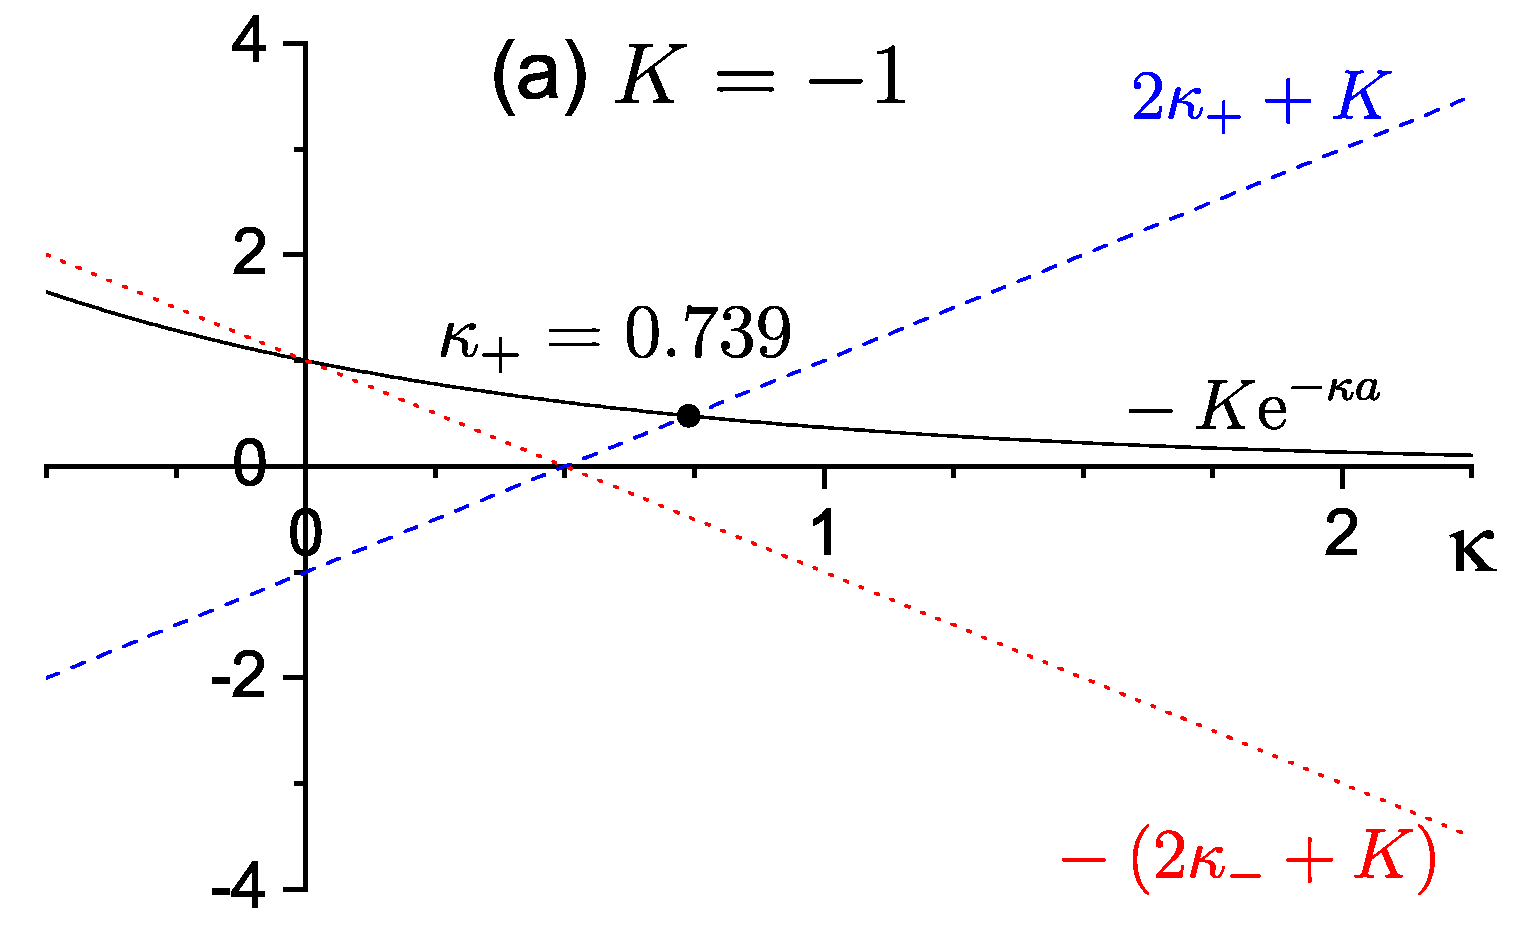
\epsfig{file=2deltak1.eps,width=\linewidth}
            \end{subfigure}
            \hfill
            \begin{subfigure}{0.49\linewidth}
                \centering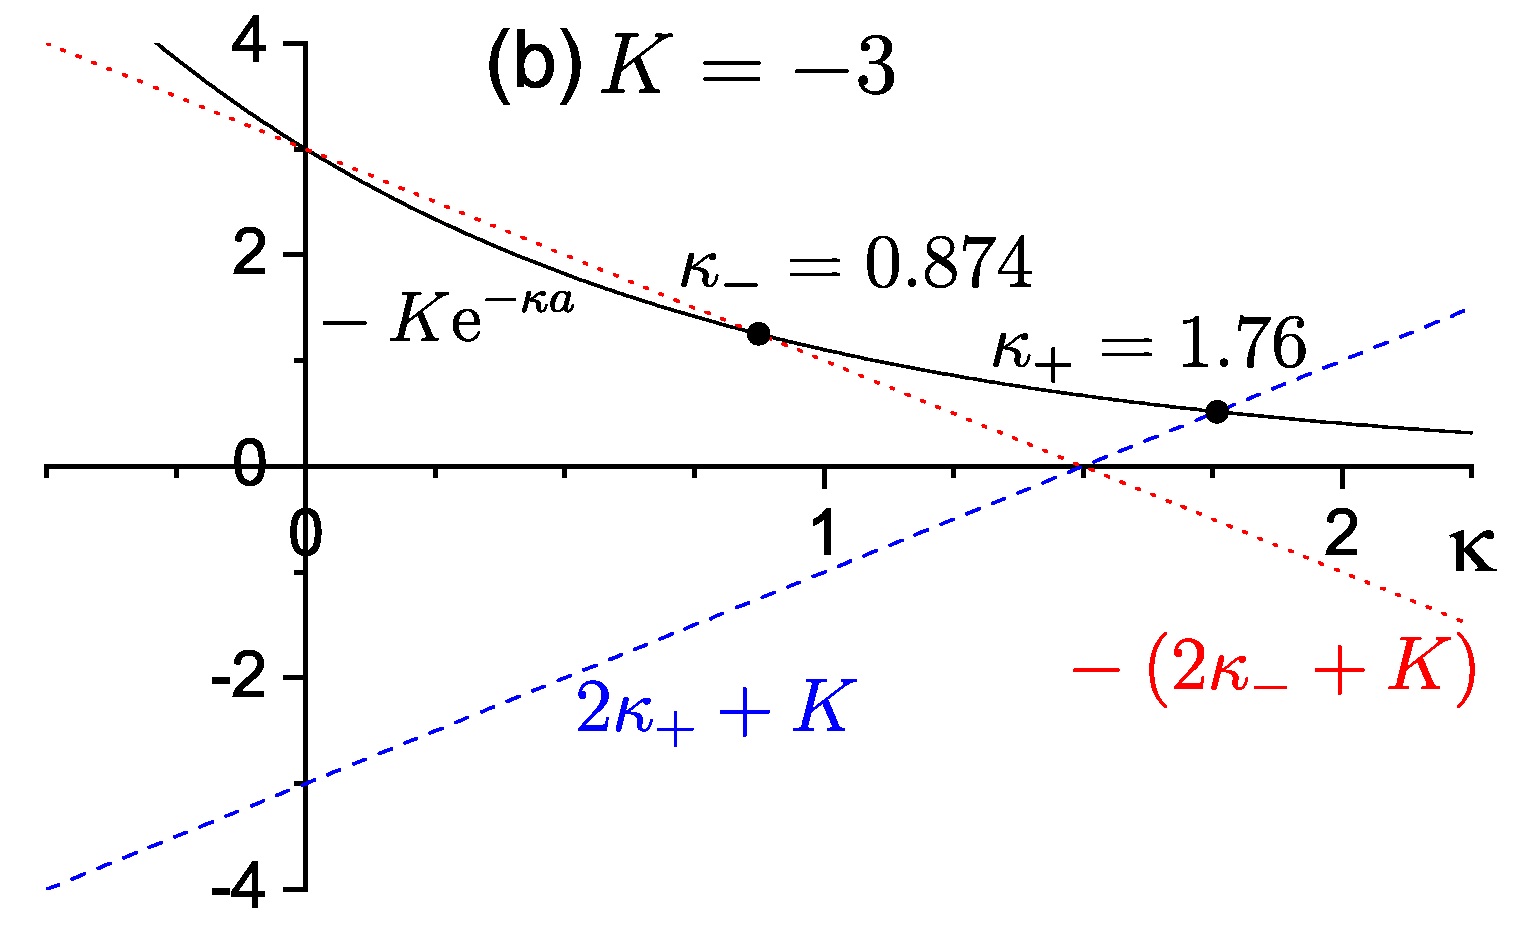
\epsfig{file=2deltak3.eps,width=\linewidth}
            \end{subfigure}
    
			\scaption{
				Numerické řešení rovnice~\eqref{eq:DoubleDeltaE} pro dvě hodnoty $K=-1$ a $K=-3$.
				V případě $K=-1$ existuje pouze sudé řešení s energií $E_{+}=-0.273$ (liché řešení $E_{-}=0$ vede na nenormalizovatelnou vlnovou funkci),
				v případě $K=-3$ existují dvě řešení $E_{+}=-1.55$ a $E_{-}=-0.382$.
			}
			\label{fig:DoubleDeltaE}
		\end{figure}		
		
		Řešení rovnic~\eqref{eq:DoubleDeltaE} lze explicitně vyjádřit pomocí \emph{Lambertových $W$ funkcí}\sfootnote{
			Lambertovy $W$ funkce jsou definovány jako řešení rovnice
			\begin{equation}
				y=x\e^{x}.
			\end{equation}
			V programu Mathematica se skrývají pod označením \href{https://reference.wolfram.com/language/ref/ProductLog.html}{ProductLog}.
		}\index{funkce!Lambertovy}
		\begin{equation}
            \kappa_{\pm}
                =-\frac{K}{2}+\frac{1}{a}\,W\left(\mp\frac{Ka}{2}\e^{\frac{Ka}{2}}\right).
		\end{equation}
		
		\begin{figure}[!htbp]
            \begin{subfigure}{0.49\linewidth}
                \centering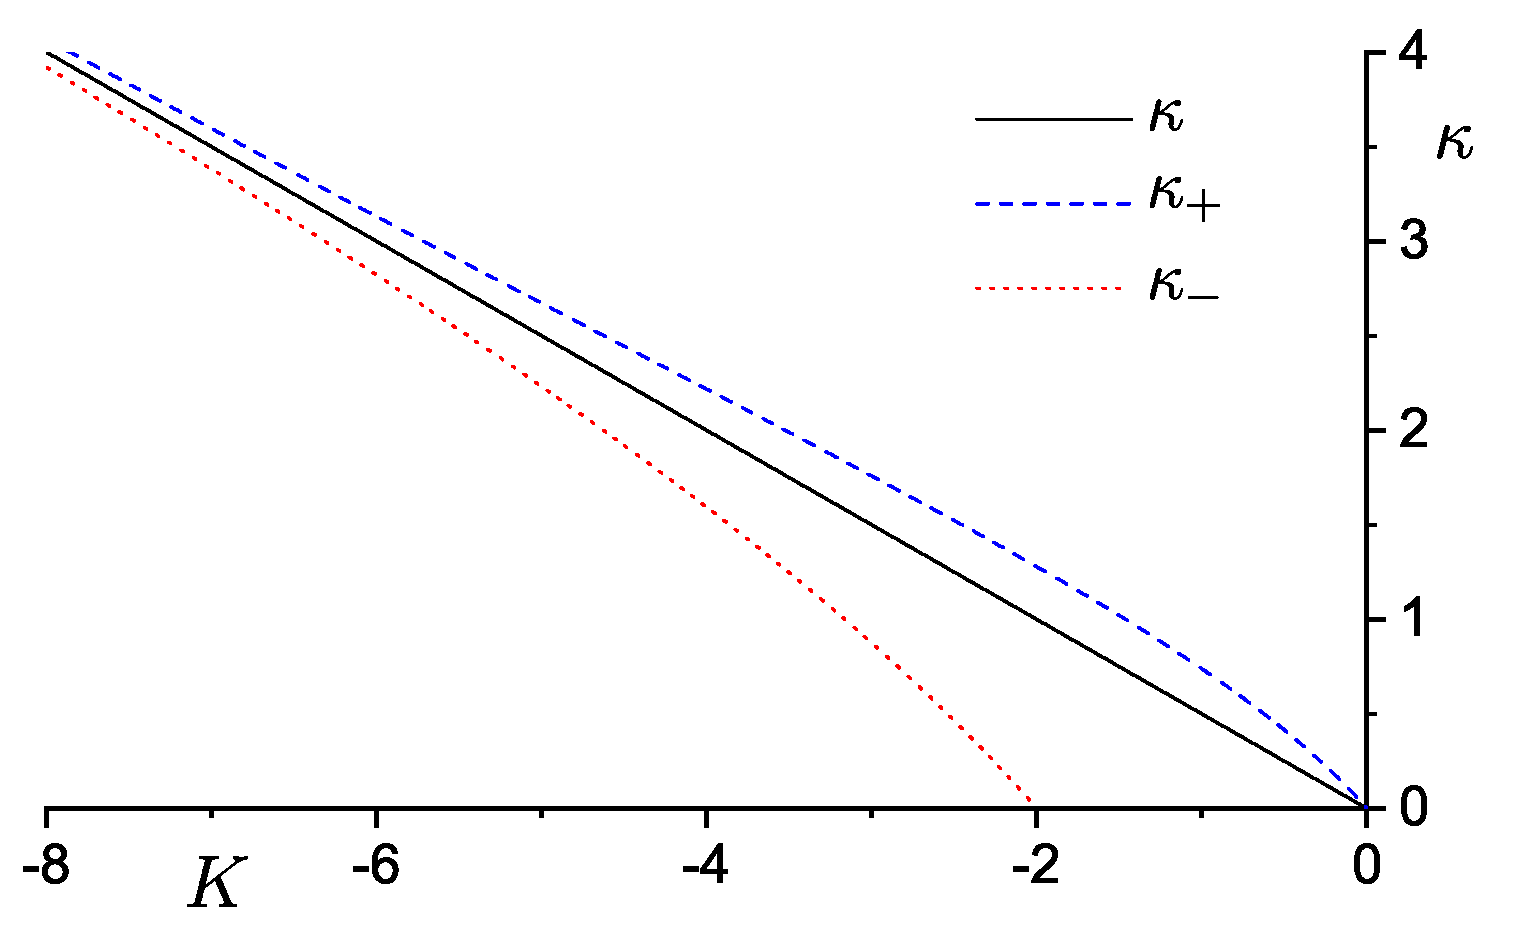
\epsfig{file=2deltaKk.eps,width=\linewidth}
            \end{subfigure}
            \hfill
            \begin{subfigure}{0.49\linewidth}
                \centering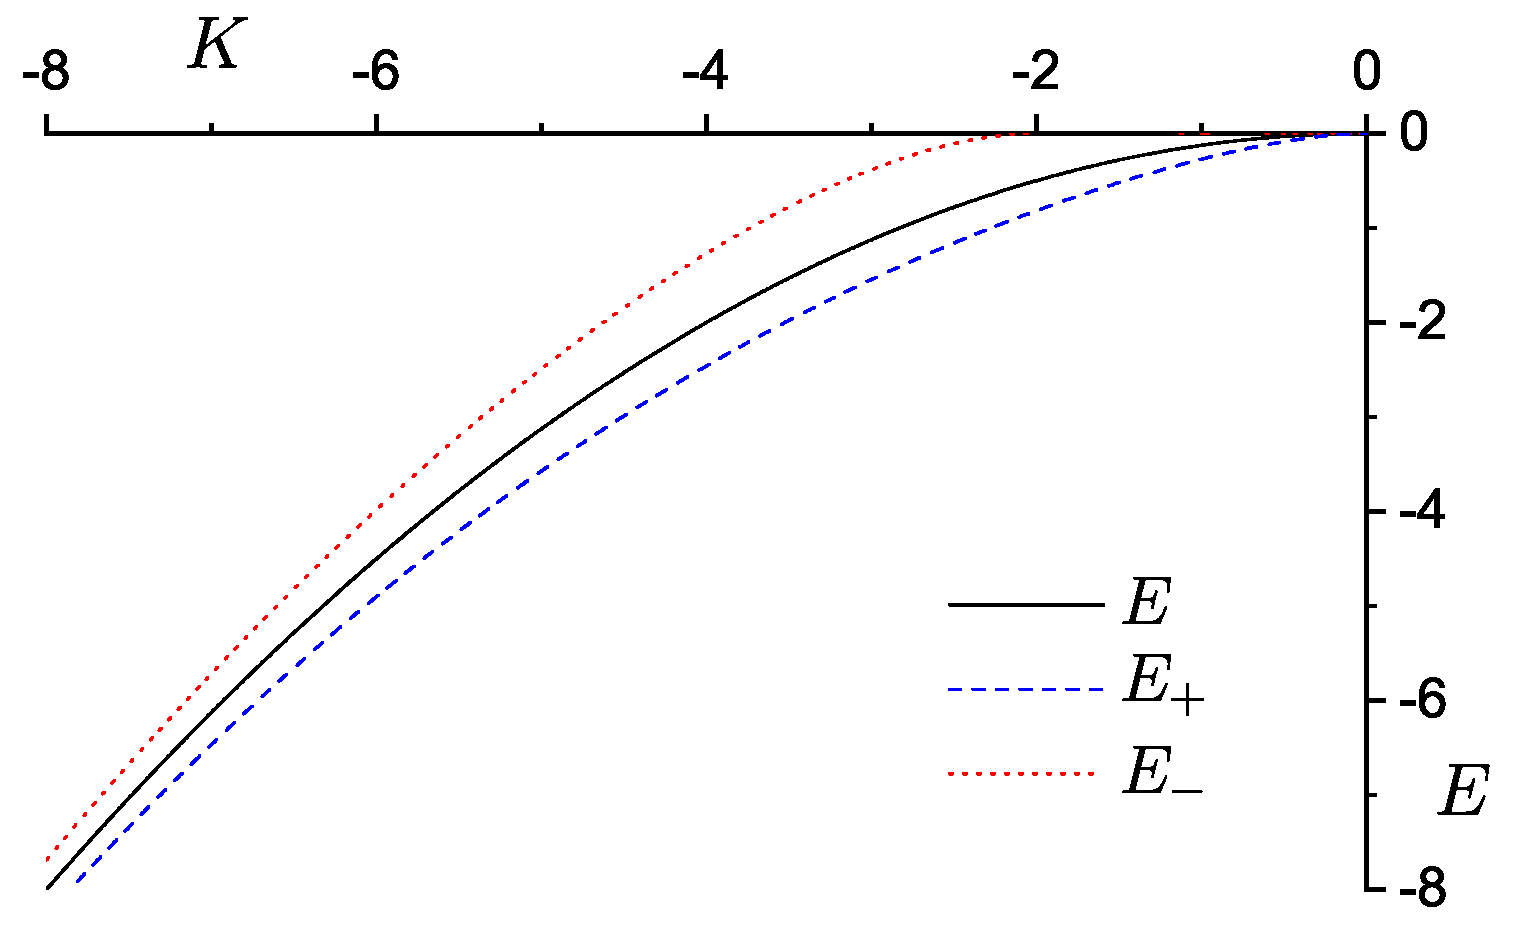
\epsfig{file=2deltaEk.eps,width=\linewidth}
            \end{subfigure}
			\scaption{
				Závislost spektra dvou $\delta$ jam $\kappa_{\pm}$ a $E_{\pm}$ na síle interakce $K$ a srovnání s jednou jámou $\kappa$ a $E$, viz~\eqref{eq:DeltaEnergy} a~\eqref{eq:DeltaK}.
			}
			\label{fig:DoubleDeltaLevelDynamics}
		\end{figure}		

		S klesající hodnotou $K$ (rostoucí silou $\delta$ funkcí v potenciálu) se řešení více a více přibližují k sobě.
		Pokud $Ka\ll0$, jámy popsané $\delta$ funkcemi mezi sebou jen velmi slabě interagují a energie budou tudíž téměř degenerované (paritní dublety) a budou blízké energii jedné $\delta$ jámy~\eqref{eq:DeltaEnergy} s dvojnásobnou silou $K$.
        Závislost řešení $\kappa_{\pm}(K)$ a odpovídajících energií $E_{\pm}(K)$ je vykreslena na obrázku~\ref{fig:DoubleDeltaLevelDynamics}.
		
		Normalizované vlnové funkce musejí splňovat normalizační podmínku
		\begin{equation}
			1=\int_{-\infty}^{\infty}\abs{\psi_{\pm}(x)}^{2}\d x
			 =2\int_{0}^{\infty}\abs{\psi_{\pm}(x)}^{2}\d x
		\end{equation}
        (druhá rovnost platí díky sudosti / lichosti vlnových funkcí).
        Sudé vlnové funkce jsou tedy
		\begin{align}
			\frac{1}{2}
				&=\int_{0}^{\frac{a}{2}}A_{+}^{2}\cosh^{2}{\kappa_{+}x}\d x
					+\int_{\frac{a}{2}}^{\infty}B_{+}^{2}\e^{-2\kappa_{+}x}\nonumber\\
				&=A_{+}^{2}\left[\frac{x}{2}+\frac{\sinh{2\kappa_{+}x}}{4\kappa_{+}}\right]
					_{0}^{\frac{a}{2}}+B_{+}^{2}\left[\frac{\e^{-2\kappa_{+}x}}{-2\kappa_{+}}\right]
					_{\frac{a}{2}}^{\infty}\nonumber\\
				&=\frac{A_{+}^{2}}{4\kappa_{+}}\left(\kappa_{+}a+\sinh{\kappa_{+}a}\right)
					+\frac{B_{+}^{2}}{2\kappa_{+}}\e^{-\kappa_{+}a}\nonumber\\
				&=\frac{A_{+}^{2}}{4\kappa_{+}}\left(\kappa_{+}a+\sinh{\kappa_{+}a}
					+2\cosh^{2}{\kappa\frac{a}{2}}\right)=\nonumber\\
				&=\frac{A_{+}^{2}}{4\kappa_{+}}\left(\e^{\kappa_{+}a}+\kappa_{+}a+1\right)
		\end{align}
		(v průběhu odvození byla použita sešívací podmínka~\eqref{eq:DoubleDeltaSewEven}), přičemž hodnoty parametrů $A_{+}$ a $B_{+}$ jsou
		\begin{subequations}
			\begin{align}
				A_{+}
					&=\sqrt{\frac{2\kappa_{+}}{\e^{\kappa_{+}a}+\kappa_{+}a+1}}
					=\sqrt{\frac{2(2\kappa_{+}+K)}{a(2\kappa_{+}+K)+2}},\nonumber\\
				B_{+}
					&=\frac{\e^{\kappa_{+}a}+1}{2}A_{+}
					=\frac{\kappa_{+}}{2\kappa_{+}+K}A_{+},
			\end{align}
		\end{subequations}
		kam se dosadilo z rovnice~\eqref{eq:kappa}.
		Liché vlnové funkce mají hodnoty parametrů
		\begin{subequations}
			\begin{align}
				A_{-}
					&=\sqrt{\frac{2\kappa_{-}}{\e^{\kappa_{-}a}-\kappa_{-}a-1}}
					=\sqrt{-\frac{2(2\kappa_{+}+K)}{a(2\kappa_{+}+K)+2}},\nonumber\\
				B_{-}
					&=\frac{\e^{\kappa_{+}a}-1}{2}A_{-}
					=-\frac{\kappa_{-}}{2\kappa_{+}+K}A_{-}.			
			\end{align}
		\end{subequations}
		Souhrnně lze tedy psát
		\begin{align}
			A_{\pm}&=\sqrt{\pm\frac{2(2\kappa_{+}+K)}{a(2\kappa_{+}+K)+2}}, & 
			B_{\pm}&=\pm\frac{\kappa_{-}}{2\kappa_{+}+K}A_{-}.			
		\end{align}
		
		\begin{figure}[!htbp]
            \begin{subfigure}{0.32\linewidth}
                \centering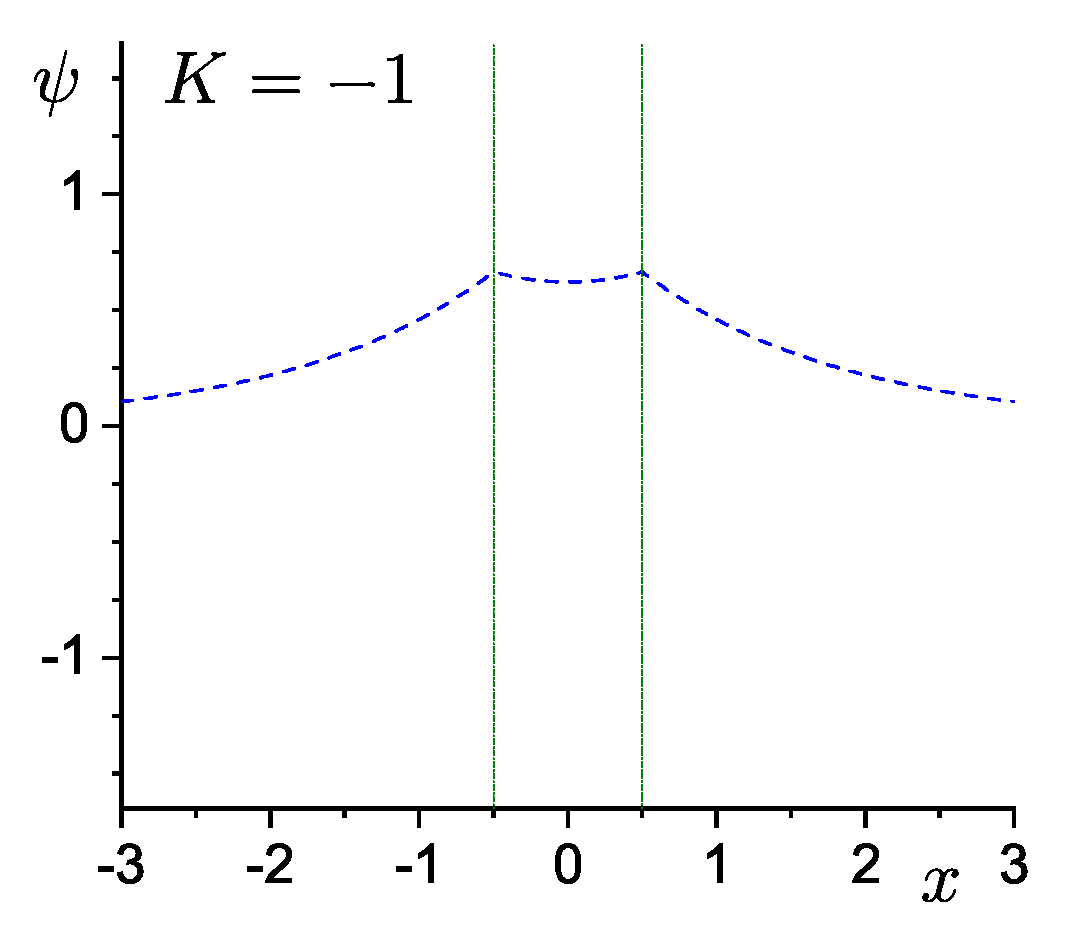
\epsfig{file=2deltapsi1.eps,width=\linewidth}
            \end{subfigure}
            \begin{subfigure}{0.32\linewidth}
                \centering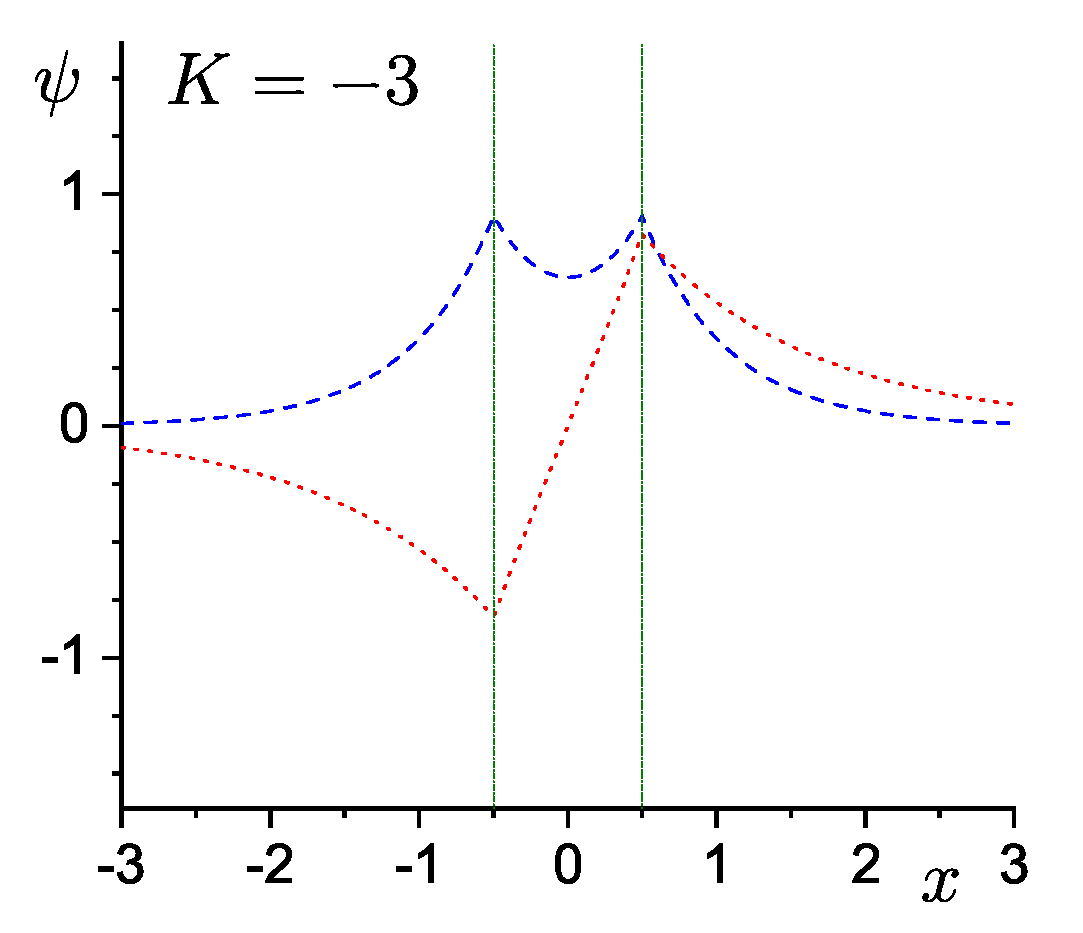
\epsfig{file=2deltapsi3.eps,width=\linewidth}
            \end{subfigure}
            \begin{subfigure}{0.32\linewidth}
                \centering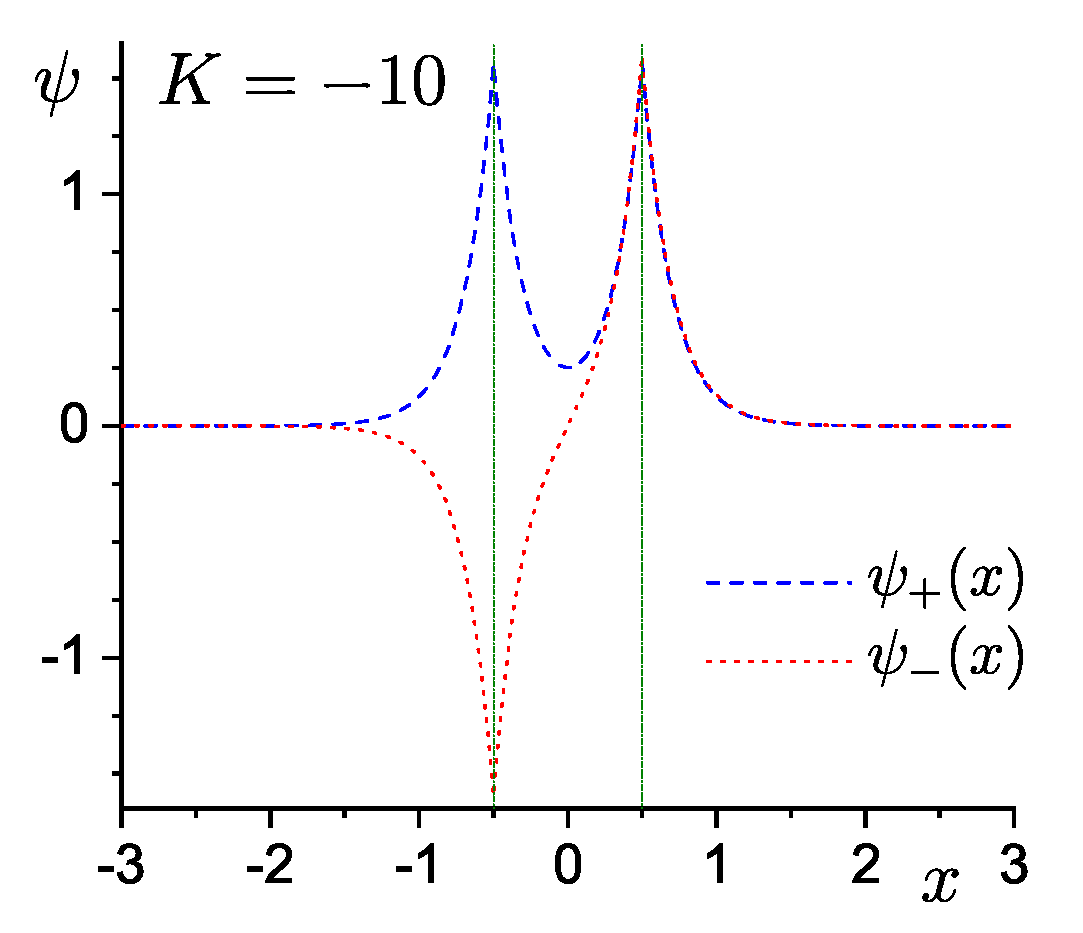
\epsfig{file=2deltapsi10.eps,width=\linewidth}
            \end{subfigure}
			\scaption{
				Normalizované vlnové funkce pro při hodnoty $K$.
				Pro $K=-1$ existuje jen jeden vázaný stav (sudá vlnová funkce), pro ostatní hodnoty $K$ existují dva vázané stavy: sudý $\psi_{+}(x)$ a lichý $\psi_{-}(x)$.
				Polohy $\delta$ funkcí jsou znázorněny svislými zelenými čerchovanými čarami.
			}
			\label{fig:DoubleDeltaWaveFunction}
		\end{figure}		

		Normalizované vlnové funkce pro tři různé hodnoty $K$ jsou zobrazeny na obrázku~\ref{fig:DoubleDeltaWaveFunction}.
		
	\item
		Pro stanovení pravděpodobnosti průchodu a odrazu se v analogii s~\eqref{eq:DeltaBarrierWF} opět vyjde z vlnové funkce ve tvaru (\trick{vlna přichází zleva})
		\begin{subequations}
			\begin{align}
				\psi_{\ti{I}}(x)
					&=A\e^{\im kx}+B\e^{-\im k x},\\
				\psi_{\ti{II}}(x)
					&=C\e^{\im kx}+D\e^{-\im k x},\\
				\psi_{\ti{III}}(x)
					&=F\e^{\im kx},
			\end{align}
		\end{subequations}
		kde $k$ je dáno vztahem~\eqref{eq:k}.
		Pravděpodobnost průchodu a odrazu bude
		\begin{equation}
            T=\abs{\frac{F}{A}}^{2},\qquad 
            R=\abs{\frac{B}{A}}^{2}.
		\end{equation}
		
		Podmínky spojitosti a skoku v derivaci vlnové funkce v bodě $\boxed{x=-a/2}$ vedou k rovnicím
		\begin{subequations}
			\begin{align}
				A\e^{-\im k\frac{a}{2}}+B\e^{\im k\frac{a}{2}}
					&=C\e^{-\im k\frac{a}{2}}+D\e^{-\im k\frac{a}{2}}\\
				\im k\left(C\e^{-\im k\frac{a}{2}}-D\e^{\im k\frac{a}{2}}
					-A\e^{-\im k\frac{a}{2}}+B\e^{+\im k\frac{a}{2}}\right)
					&=K\left(A\e^{-\im k\frac{a}{2}}+B\e^{\im k\frac{a}{2}}\right).		
			\end{align}
		\end{subequations}
		Z první rovnice vynásobené faktorem ${\im k}$ se vyjádří
		\begin{equation}\label{eq:DoubleDeltaCD1}
            C\im k\e^{-\im k\frac{a}{2}}
                =\im k\left(A\e^{-\im k\frac{a}{2}}+B\e^{\im k\frac{a}{2}}-D\e^{\im k\frac{a}{2}}\right)
		\end{equation}
		a tento výraz se dosadí do druhé rovnice, což po úpravách dá
		\begin{equation}
            \im k\left(B\e^{\im k\frac{a}{2}}-D\e^{\im k\frac{a}{2}}\right)
                =\frac{K}{2}\left(A\e^{-\im k\frac{a}{2}}+B\e^{\im k\frac{a}{2}}\right),
		\end{equation}
		a tedy
		\begin{equation}\label{eq:DoubleDeltaD1}
			D=\frac{\im K}{2k}\left(A\e^{-\im ka}+B\right)+B.
		\end{equation}
		Zpětným dosazením do~\eqref{eq:DoubleDeltaCD1} se dostane
		\begin{equation}\label{eq:DoubleDeltaC1}
			C=A-\frac{\im K}{2k}\left(A+B\e^{\im ka}\right).
		\end{equation}
		
		Analogický postup se zopakuje v bodě $\boxed{x=a/2}$, případně stačí vzít výsledek~\eqref{eq:DoubleDeltaD1} 
		a~\eqref{eq:DoubleDeltaC1} a provést záměnu $k\mapsto-k$, $A\mapsto F$, $B\mapsto 0$:
		\begin{align}\label{eq:DoubleDeltaCD2}
			C&=\frac{-K+2\im k}{2\im k}F &
			D&=-\frac{\im K}{2k}F\e^{\im ka}.
		\end{align}
		Zkombinování vztahů~\eqref{eq:DoubleDeltaD1}, \eqref{eq:DoubleDeltaC1} a \eqref{eq:DoubleDeltaCD2} vede na soustavu dvou rovnic pro neznámé $B$ a $E$:
		\begin{subequations}
			\begin{align}
				\frac{\im K}{2k}\left(A\e^{-\im ka}+B\right)+B
					&=-\frac{\im K}{2k}F\e^{\im ka},\\
				A-\frac{\im K}{2k}\left(A+B\e^{-\im ka}\right)
					&=\frac{-K+2\im k}{2\im k}F.
			\end{align}
		\end{subequations}
		Bez újmy na obecnosti lze volit $A=1$, čímž se vztahy pro pravděpodobnosti průchodu a odrazu zjednoduší na $T=\abs{F}^{2}$ a $R=\abs{B}^{2}$.
		
		Řešení posledních dvou rovnic zní
		\begin{equation}
			F=\frac{4k^{2}}{K^{2}\e^{2\im ka}-\left(K-2\im k\right)^{2}}.
			\label{eq:2DeltaF}
		\end{equation}
		Po úpravách se získá finální výraz pro pravděpodobnost průchodu
		\begin{align}
			T&=FF^{*}
				=\frac{4k^{2}}{K^{2}\e^{2\im ka}-\left(K-2\im k\right)^{2}}
					\frac{4k^{2}}{K^{2}\e^{-2\im ka}-\left(K+2\im k\right)^{2}}\nonumber\\
			 &=\frac{16k^{4}}{\underbrace{\left(K^{2}+4k^{2}\right)^{2}+K^{4}}
				_{2\clubsuit=2K^{4}+8K^{2}k^{2}+16k^{4}}-K^{2}\left[(K+2\im k)^{2}\e^{2\im ka}
				+\left(K-2\im k\right)^{2}\e^{-2\im ka}\right]}\nonumber\\
			 &=\frac{16k^{4}}{2\clubsuit-K^{2}\left[\left(K^{2}-4k^{2}\right)
				\left(\e^{2\im ka}+\e^{-2\im ka}\right)+4\im Kk\left(\e^{2\im ka}
				-\e^{-2\im ka}\right)\right]}\nonumber\\
			 &=\frac{16k^{4}}{2\clubsuit-K^{2}\left[2\left(K^{2}-4k^{2}\right)\cos{2ka}
				-8Kk\sin{2ka}\right]}\nonumber\\
			 &=\frac{8k^{4}}{\clubsuit-K^{2}\left[\left(K^{2}-4k^{2}\right)
				\left(\cos^{2}ka-\sin^{2}ka\right)-8Kk\sin{ka}\cos{ka}\right]}\nonumber\\
			 &=\frac{8k^{4}}{\clubsuit-K^{4}\cos^{2}ka+K^{4}\sin^{2}ka+4K^{2}k^{2}\cos^{2}ka
				-4K^{2}k^{2}\sin^{2}ka+8K^{3}k\sin{ka}\cos{ka}}\nonumber\\
			 &=\frac{4k^{4}}{4k^{4}+2K^{4}\sin{2}ka+8K^{2}k^{2}\cos^{2}ka
				+8K^{3}k\sin{ka}\cos{ka}}\nonumber\\
			 &=\frac{4k^{4}}{4k^{4}+K^{2}\left(K\sin{ka}+2k\cos{ka}\right)^{2}}\nonumber\\
			 &=\frac{1}{1+\frac{K^{2}}{4k^{2}}\left(2\cos{ka}+\frac{K}{k}\sin{ka}\right)^{2}}.
		\end{align}
        
        Srovnání s pravděpodobností průchodu pro jednu $\delta$ funkci~\eqref{eq:DeltaT} ukazuje, že v případě dvou $\delta$ funkcí se $T$ liší o modulační faktor v závorce ve jmenovateli.
		Ten způsobuje, že pro speciální hodnoty $k$ dané rovnicí
		\begin{equation}
			2\cos{ka}+\frac{K}{k}\sin{ka}=0,
		\end{equation}
		tj.
		\begin{equation}
            \tan{ka}
                =-\frac{2k}{K}
		\end{equation}		
		je pravděpodobnost průchodu $T=1$ a pravděpodobnost odrazu $R=0$.
		To je speciální případ tzv.~\emph{Ramsauerova-Townsendova efektu}\index{efekt!Ramsauerův-Townsendův}, viz též~\cite{Capri2002}, kapitola 4.10.
		Pravděpodobnost průchodu $T$ je pro dvě hodnoty $K$ zobrazena na obrázku~\ref{fig:DoubleDelta}~(a) a srovnána s případem pravděpodobnosti průchodu pro jednu $\delta$ funkci~\eqref{eq:DeltaT} s dvojnásobnou silou $K$ (limitní případ $a\rightarrow0$).
		Pravděpodobnost odrazu se dopočítá pomocí relace $R=1-T$.	
		
	\item
		Fázové posunutí se spočítá pomocí definičního vztahu~\eqref{eq:PhaseShift} z výrazu~\eqref{eq:2DeltaF}:
		\begin{align}
            F&=\frac{4k^{2}}{K^{2}\left(\cos{2ka}+\im\sin{2ka}\right)-\left(K-2\im k\right)^{2}}\nonumber\\
			 &=\frac{4k^{2}}{K^{2}(\cos{2ka}-1)+4k^{2}+\im K(K\sin{2ka}+4k)}\nonumber\\
			 &=\frac{4k^{2}\left[K^{2}(\cos{2ka}-1)+4k^{2}-\im K\left(K\sin{2ka}+4k\right)\right]}{\left[K^{2}(\cos{2ka}-1)+4k^{2}\right]^{2}+K^{2}\left(K\sin{2ka}+4k\right)^{2}},
		\end{align}
		\begin{equation}
			\delta=-\arctan\frac{\sin{2ka}+\frac{4k}{K}}{\cos{2ka}-1+\frac{4k^{2}}{K^{2}}}.
		\end{equation}
		Fázové posunutí je zobrazeno na obrázku~\ref{fig:DoubleDelta}~(b).
		Přitažlivý potenciál ($K<0$) dává fázové posunutí záporné, odpudivý potenciál ($K>0$) kladné.
		
		\begin{figure}[!htbp]
            \begin{subfigure}{0.49\linewidth}
                \centering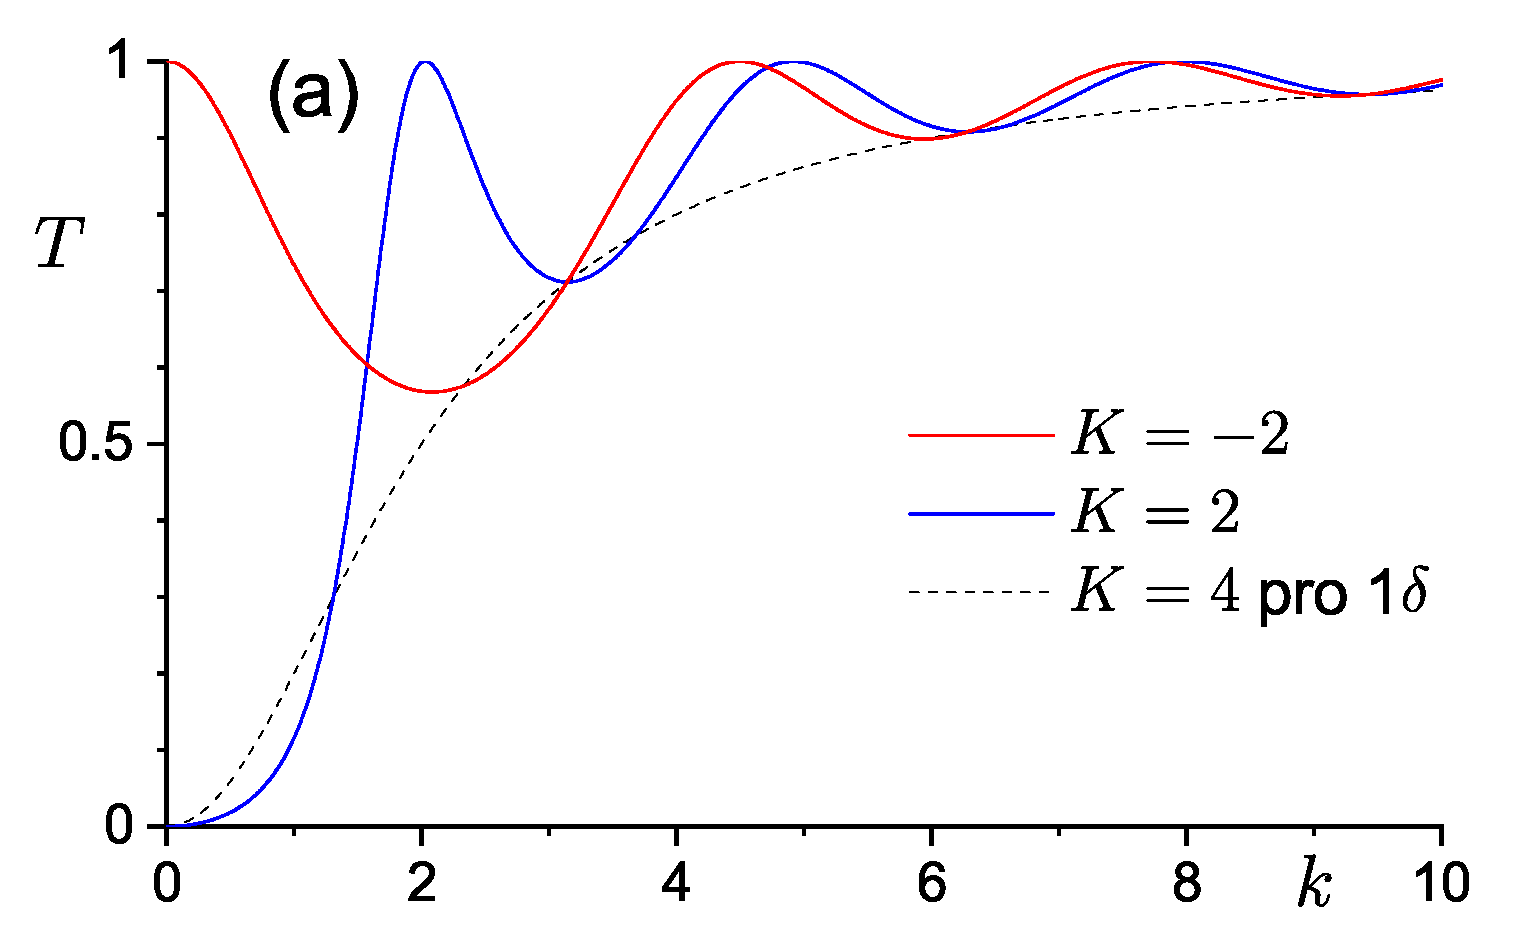
\epsfig{file=2deltaT.eps,width=\linewidth}
            \end{subfigure}
            \hfill
            \begin{subfigure}{0.49\linewidth}
                \centering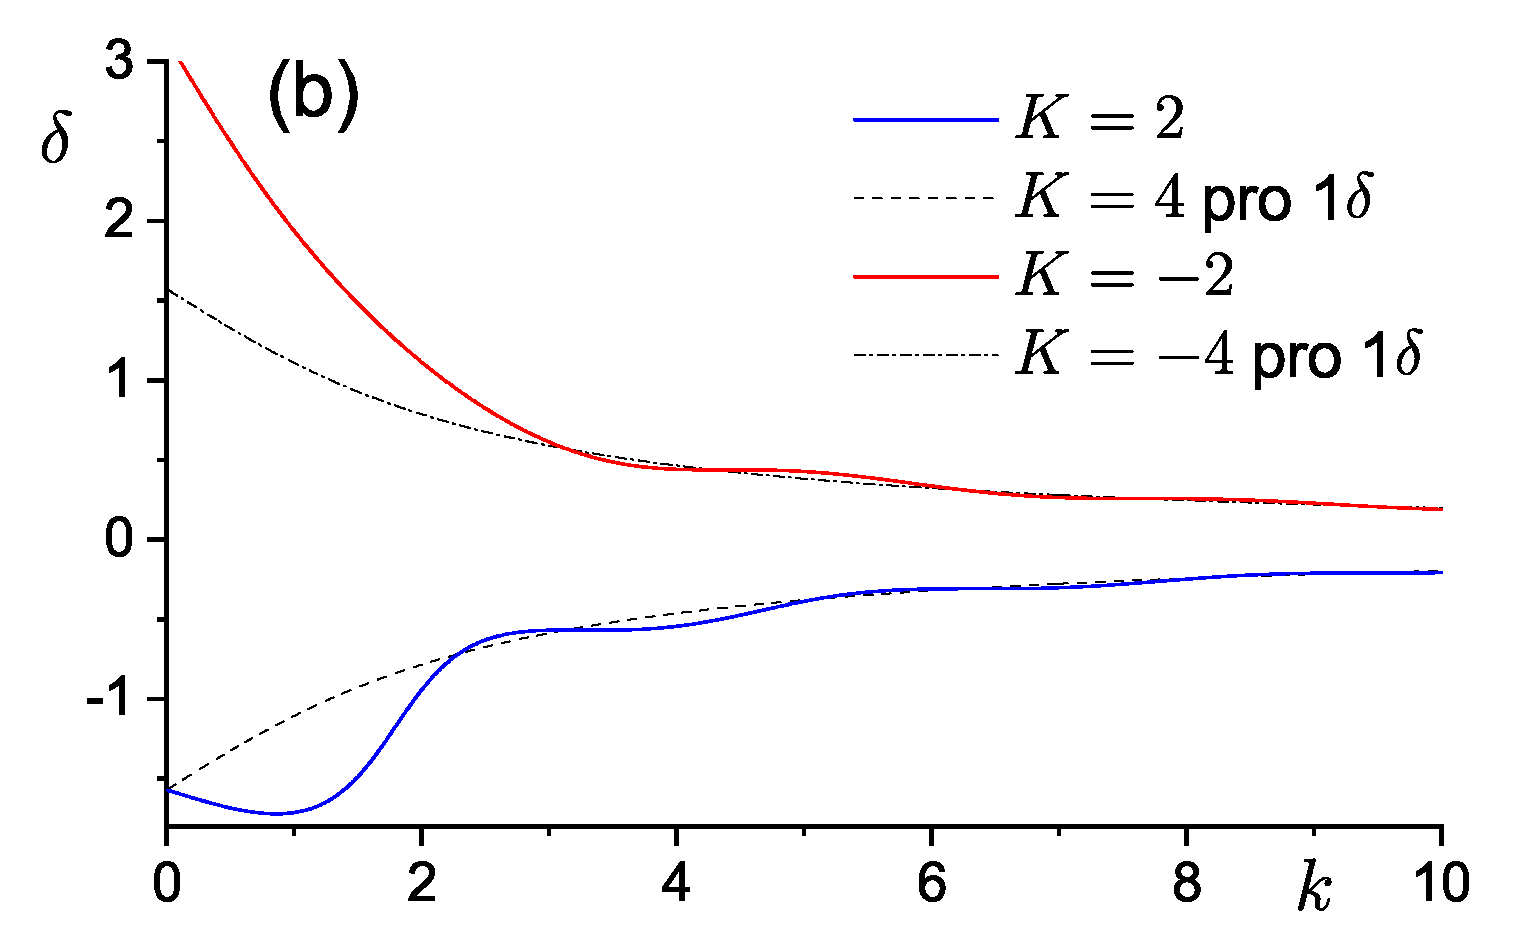
\epsfig{file=2deltadelta.eps,width=\linewidth}
            \end{subfigure}
			\scaption{
				(a) Pravděpodobnost průchodu a (b) fázové posunutí $\delta$ pro potenciál dvou $\delta$ jam s $K=-2$ (červeně) a $K=2$ (modře).
				Pro srovnání s případem jedné jámy síly $K=\pm4$ slouží černá čárkovaná čára 
				(v případě jedné jámy je pravděpodobnost průchodu stejná pro obě znaménka $K$).
			}			
			\label{fig:DoubleDelta}
		\end{figure}		
				
	\end{enumerate}
\end{solution}